\documentclass{article}[18pt]
\usepackage{../../../../format}
\lhead{Networks and Systems - Networks}


\begin{document}
\begin{center}
\underline{\huge Physical Layer}
\end{center}
\section{Bandwidth}
Bandwidth is the physical property fo the transmission medium
\begin{defin}[Baseband]
	The signal that runs from 0 to a maximum frequency. Has very narrow and near-zero frequency range. Used in wires
\end{defin}
\begin{defin}[Passband]
	Signals that occupy the higher range of frequency and pass through frequency filter(s). Used in wireless spectrum
\end{defin}
\subsection{Signal Bandwidth}
Bandwidth of analogue and digital signals are measured differently:
\begin{itemize}
	\item Analogue signal bandwidth is measured in terms of its frequency (Hz)
	\item Digital signal bandwidth is measured in terms of bit rate (bps)
\end{itemize}
\section{Digital Modulation}
Digital signals (0,1) are encoded by low and high voltage\\
\\
There are many digital encoding schemes
\begin{center}
	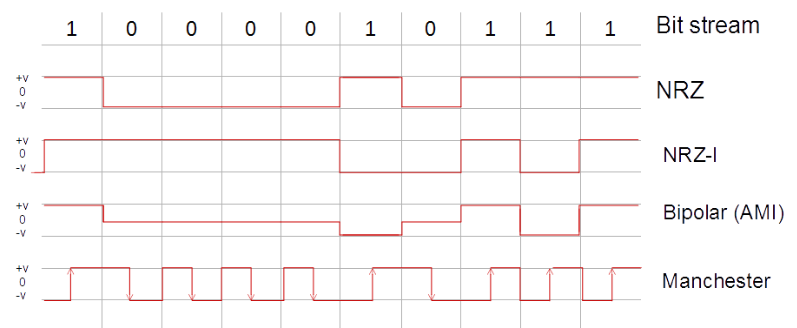
\includegraphics[scale=0.7]{Modulation}
\end{center}
\subsection{NRZ Encoding (Non-Return-to-Zero)}
\begin{itemize}
	\item A high voltage represents a 1 and a low voltage represents a 0
	\item The voltage does not return to zero, it changes only when the bit value changes
\end{itemize}
\begin{itemize}
	\item Problem: having long runs of consecutive bits with the same value (no changes in voltage) the constant signal values can't synchronize the communicating devices
\end{itemize}
\subsection{NRZI Encoding}
\begin{itemize}
	\item NRZI attempts to alleviate the problem in NRZ scheme
	\item 0 is encoded as no change in the level. 1 is encoded depending on the current state of the line
	\item If the current state is low voltage the 1 will be encoded as high voltage, if the current state is again high voltage the 1 will be encoded as a low voltage
\end{itemize}
\begin{itemize}
	\item This fixes the problem of sending consecutive 1s but not consecutive 0s
\end{itemize}
\subsection{Bipolar Encoding}
\begin{itemize}
	\item 0 is represented by a zero voltage, neither high nor low
	\item 1 is represented by either positive voltage or negative voltage
	\begin{itemize}
		\item It is inverted based on the last transmission of 1
		\item It is represented by a negative voltage if it was represented by a positive voltage when it was last transmitted, and vice versa
	\end{itemize}
\end{itemize}
\subsection{Manchester Encoding}
\begin{itemize}
	\item Manchester code: a high to low voltage represents a 1 and a low to high voltage represents a 0
	\item Uses signal changes to transmit a bit and achieves synchronisation
	\item Twice the bandwidth of NRZ is required
\end{itemize}
\section{Multiplexing}
\begin{itemize}
	\item Channels are often shared by multiple signals
	\item Different ways to accomplish multiplexing:
\end{itemize}
\subsection{Frequency Division Multiplexing}
\begin{center}
	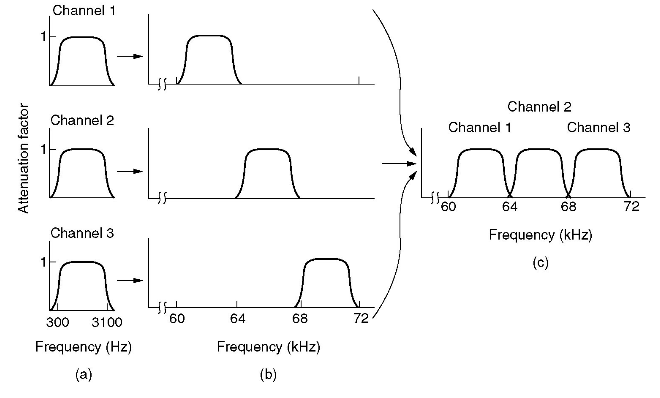
\includegraphics[scale=0.7]{FDM}
\end{center}
\begin{enumerate}[label=\alph*]
	\item The original bandwidths
	\item The bandwidths raised in frequency
	\item The multiplexed channel
\end{enumerate}
\subsection{Wavelength Division Multiplexing}
\begin{center}
	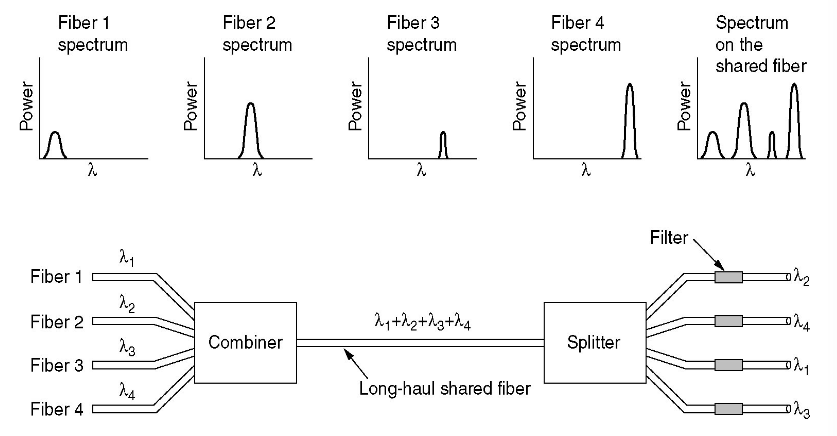
\includegraphics[scale=0.7]{WDM}
\end{center}
\subsection{Time division multiplexing}
\begin{center}
	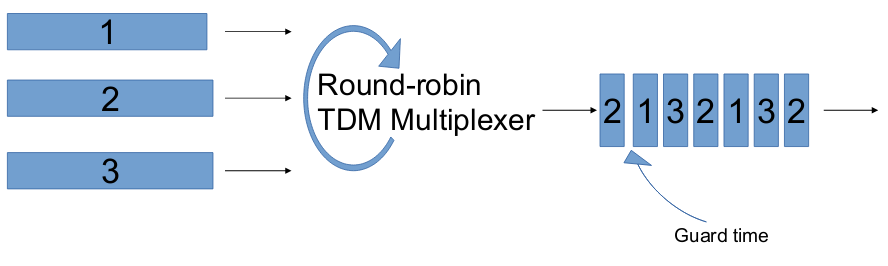
\includegraphics[scale=0.7]{TDM}
\end{center}
\subsection{Code Division Multiple Access}
\begin{itemize}
	\item Nice and clean mathematical method allows every transmitter to use the entire channel all the time
	\item The individual transmissions are blended (or extracted by a receiver) using coding theory
	\item Imagine that we have four transmitters called, from now on, stations
	\item Each station has a chip, which is a four bit vector
\end{itemize}


\end{document}